%% LyX 2.1.2.2 created this file.  For more info, see http://www.lyx.org/.
%% Do not edit unless you really know what you are doing.
\documentclass{article}
\usepackage[latin9]{inputenc}
\usepackage[tmargin=2cm,bmargin=2cm,lmargin=3cm,rmargin=3cm]{geometry}
\usepackage{amstext,amsmath}
\usepackage{graphicx}
% \usepackage{babel}
\usepackage{dsfont}

\newcommand{\var}{\mbox{var}}
\newcommand{\E}{\mbox{E}}

\begin{document}
\begin{center}
\hrule \vspace{3mm}
	{\Large Exam : Statistical modelling and its applications}\\ \vspace{3mm}
	{Mines Saint-\'Etienne -- 5th January 2016} \\  \vspace{2mm}
	{\footnotesize No document allowed except the Gaussian process regression handout and an A4 sheet with hand written notes.}\\ \vspace{3mm}
	\hrule
\end{center}
\vspace{5mm}
%%%%%%%%%%%%%%%%%%%%%%%%%%%%%%%%%%%%%%%%%%%%%%%%%%%%%%%%%%%%%%%%%%%%
%%%%%%%%%%%%%%%%%%%%%%%%%%%%%%%%%%%%%%%%%%%%%%%%%%%%%%%%%%%%%%%%%%%%
\section*{Exercise 1 (5 pts)}

\begin{enumerate}
\item {[1 pt]} Detail how to generate samples from a one-dimensional Gaussian process with mean $\mu(.)$ and kernel $k(.,.)$.
\item {[1.5 pts]} The following figures show samples from four Gaussian processes. For each one, specify
\begin{itemize}
	\item the kernel (either exponential, Brownian, squared exponential or Mat\'ern 3/2),
	\item if the process is centred (yes/no),
	\item if the process is stationary (yes/no).
\end{itemize}
\begin{center}
	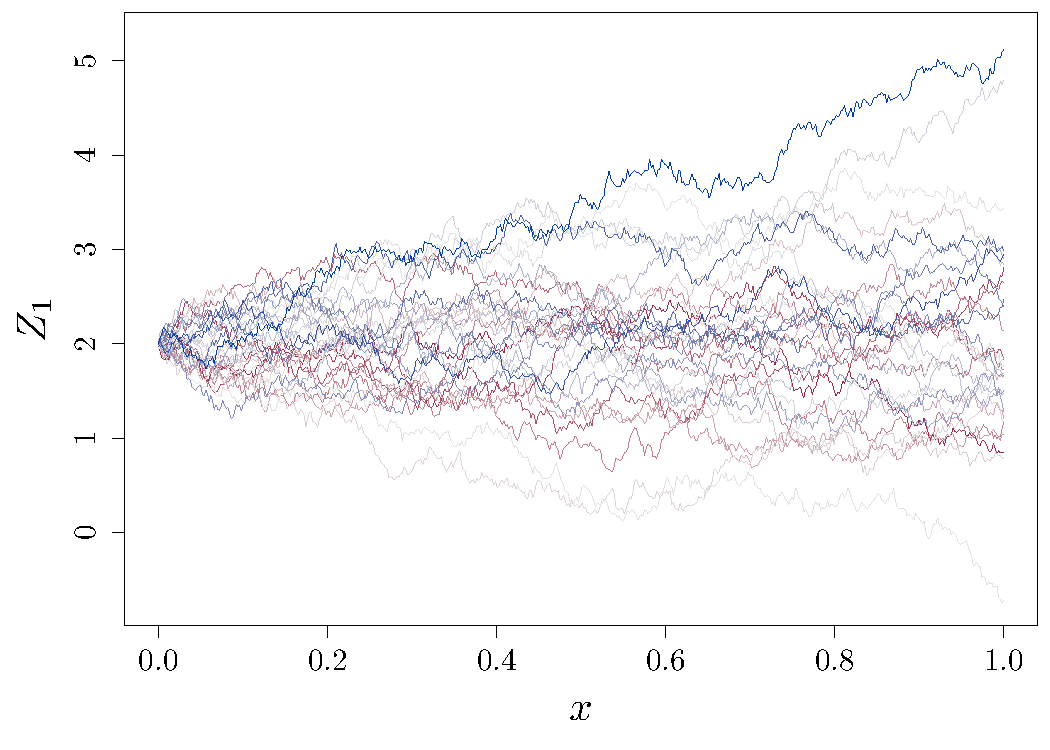
\includegraphics[width=5cm]{figures/GPR_simBrown.pdf} \qquad
	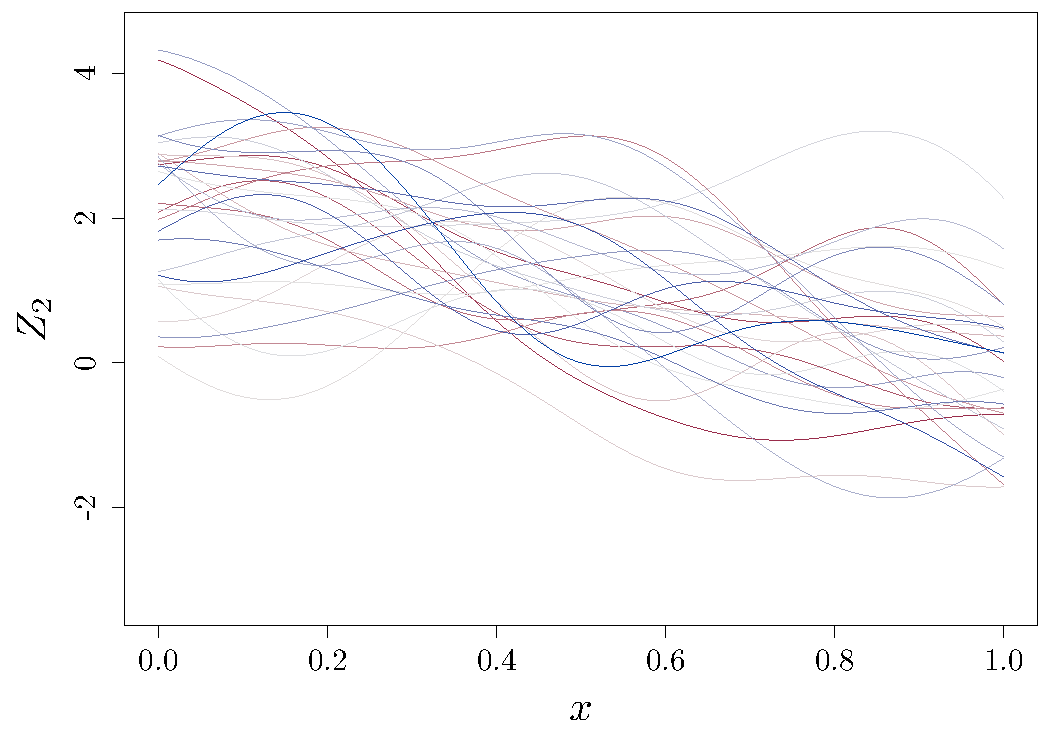
\includegraphics[width=5cm]{figures/GPR_simGauss.pdf}\\
	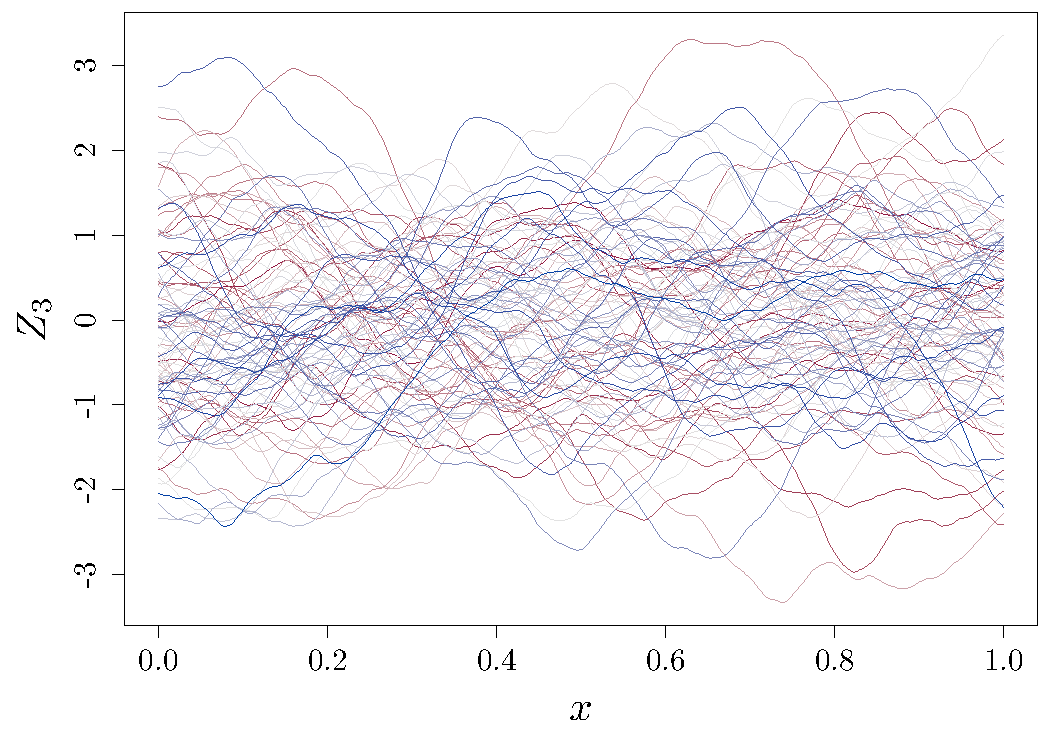
\includegraphics[width=5cm]{figures/GPR_simMat.pdf} \qquad
	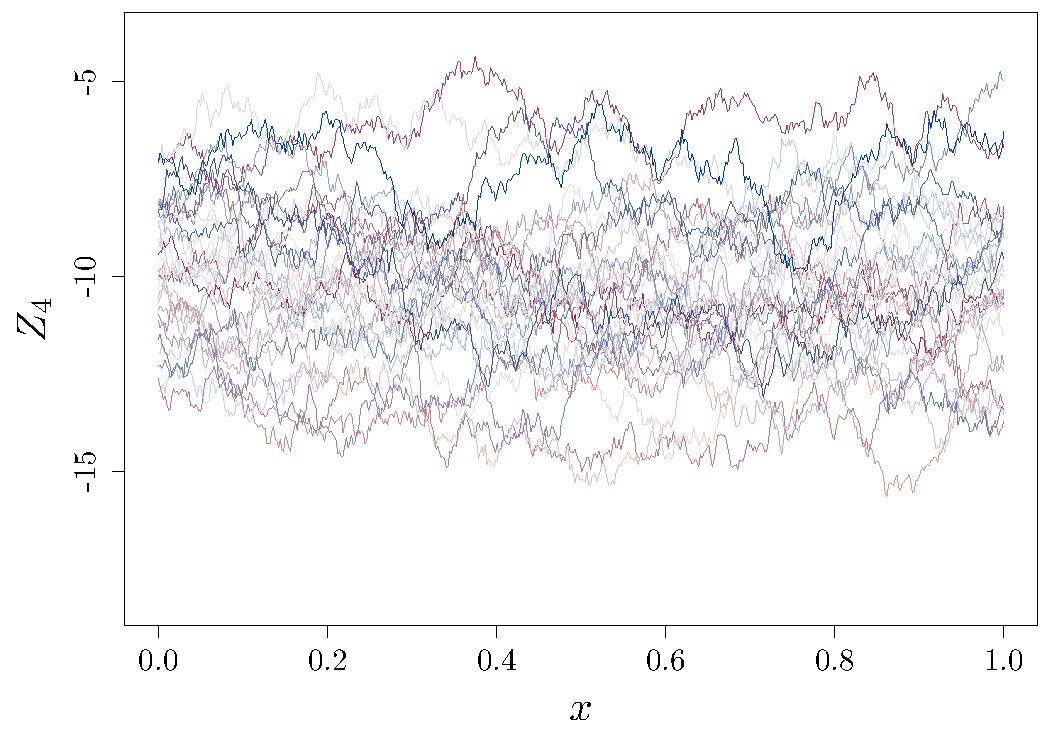
\includegraphics[width=5cm]{figures/GPR_simExp.pdf}
\end{center}
\item{[1 pt]} The figures bellow correspond to samples of a Matern 5/2 kernel with variance parameter $\sigma^2 \in \{0.1, 1, 10, 100 \}$ and with length scale $\theta \in \{0.1,1,10\}$. For each figure, specify the corresponding set of parameters.
\begin{center}
	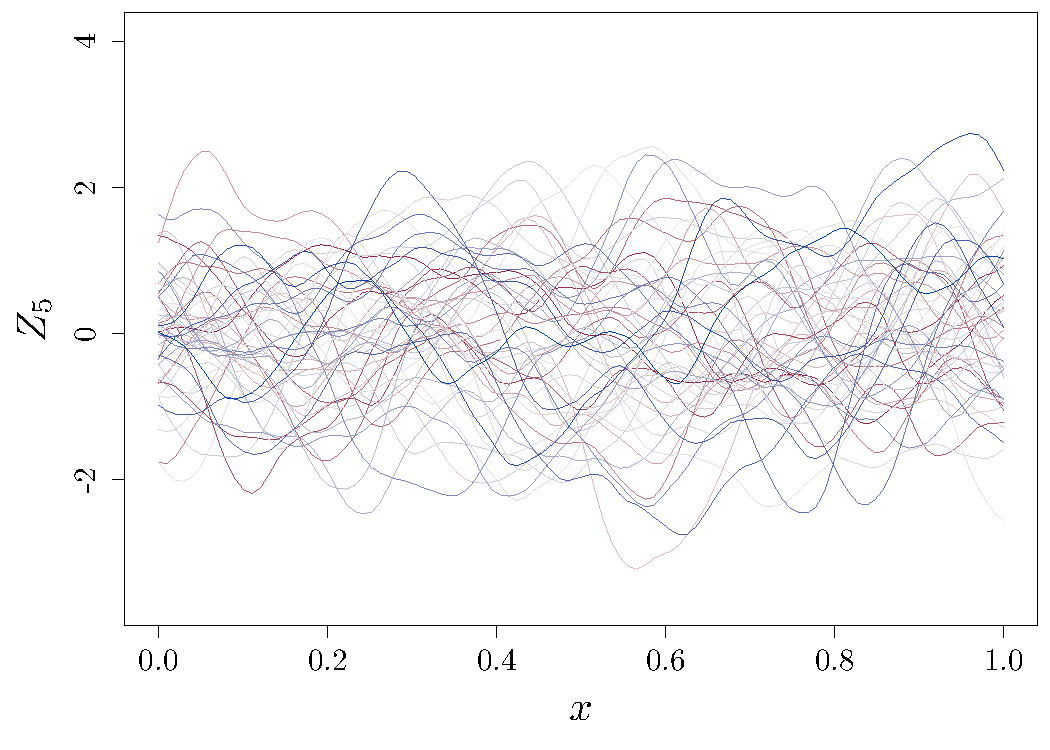
\includegraphics[width=5cm]{figures/GPR_simMat52_1_01.pdf} \qquad
	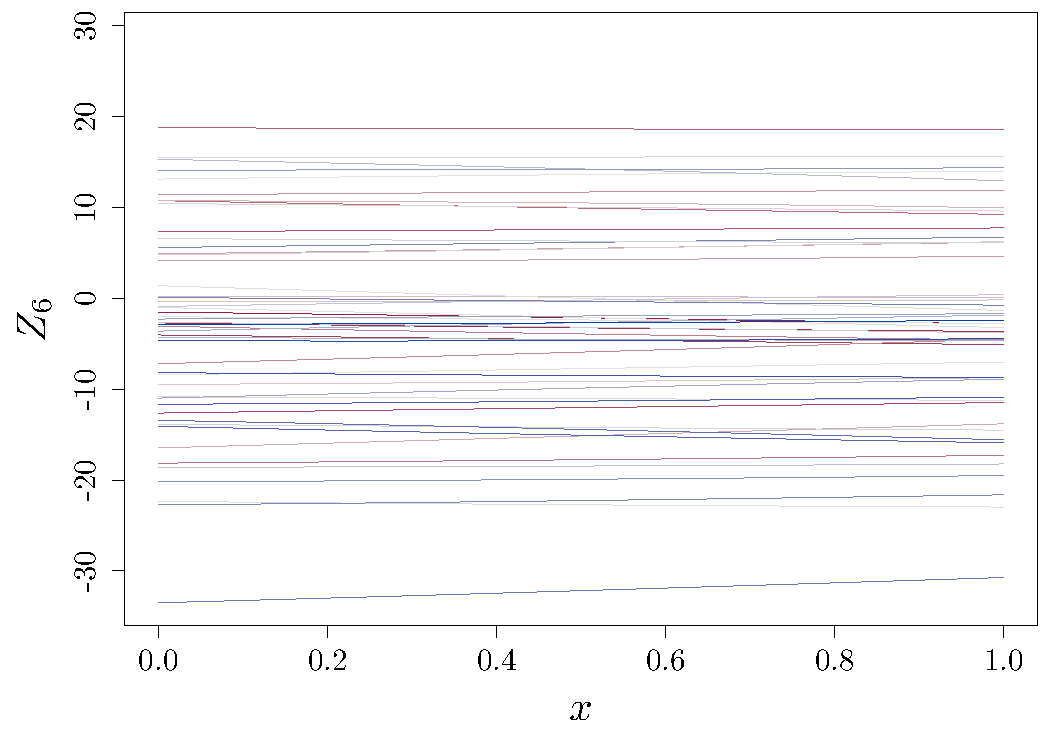
\includegraphics[width=5cm]{figures/GPR_simMat52_100_10.pdf} \\
\end{center}
\item {[1.5 pts]} We are interested in computing the mean value of a function $f$ using no more that 50 observations. What are the main steps you would go through for solving this problem.
\end{enumerate} 

\newpage
%%%%%%%%%%%%%%%%%%%%%%%%%%%%%%%%%%%%%%%%%%%%%%%%%%%%%%%%%%%%%%%%%%%%
%%%%%%%%%%%%%%%%%%%%%%%%%%%%%%%%%%%%%%%%%%%%%%%%%%%%%%%%%%%%%%%%%%%%
\section*{Exercise 2 (7 pts)}
Let us consider the 2-dimensional function: $f(x_{1},x_{2})= x_1 + x_2 + x_1 x_2$.\\

\noindent
The aim is to perform a global sensitivity analysis of $f(X_{1},X_{2})$
where $X_{1}$, $X_{2}$ are independent uniform random variables, 
with $X_1 \sim \mathcal{U} \left[-\frac{a}2,\frac{a}2 \right]$  and  $X_2 \sim \mathcal{U}[-\frac{1}2,\frac{1}2]$,
and $a>0$.\\

\noindent We recall that for a uniform random variable $Z \sim \mathcal{U}[s,t]$, 
we have $\E(Z)= \frac{s+t}2$ and $\var(Z) = \frac{(t-s)^2}{12}$.\\

\begin{enumerate}
\item {[}2 pts{]} By verifying that $X_1$, $X_2$ and $X_1X_2$ satisfy the centering and non-simplification conditions,
show that the Sobol-Hoeffding decomposition of $f(X_1, X_2)$ is simply:
$$\mu_0 = 0, \quad  \mu_1(X_1) = X_1, \quad \mu_2(X_2) = X_2, \quad \mu_{1,2}(X_1, X_2) = X_1X_2$$
\item {[}1.5 pts{]} Compute the partial variances $D_I = \var(\mu_I(X_I))$ for $I = \{1\}, \{2\}, \{1,2\}$ 
and check that the global variance is $D = \var(f(X_1, X_2)) = \frac{1}{12} \left( 1 + \frac{13}{12} a^2 \right)$ 
\item {[}1.5 pts{]} Recall that Sobol indices are defined by $S_I = D_I/D$. Compute $S_1$ and $S_2$, 
and check that $S_1$ (resp. $S_2$) is an increasing (resp. decreasing) function of $a$. Interpretation?\\
\end{enumerate} 

\noindent We now assume that $X_{1}$, $X_{2}$ are independent random variables, with $X_1, X_2 \sim \mathcal{U}[0, 1]$.\\

\begin{enumerate}
\setcounter{enumi}{3}
\item {[}0.5 pt{]} Explain why it is now \textit{wrong} that $\mu_1(X_1) = X_1$.
\item {[}1.5 pts{]} Compute the Sobol decomposition of $f(X_1, X_2)$. 
\end{enumerate}

%%%%%%%%%%%%%%%%%%%%%%%%%%%%%%%%%%%%%%%%%%%%%%%%%%%%%%%%%%%%%%%%%%%%
%%%%%%%%%%%%%%%%%%%%%%%%%%%%%%%%%%%%%%%%%%%%%%%%%%%%%%%%%%%%%%%%%%%%
\section*{Exercise 3: ANOVA kernels (8 pts)}
ANOVA kernels are kernels over $\mathds{R}^d \times \mathds{R}^d$ of the form : $ k(x,y) = \prod_{i=1}^d  \big(1+k_i(x_i,y_i) \big)$, where the $k_i$ are symmetric positive semi-definite functions.

\begin{enumerate}
\item{[1 pt]} Using the results from the course, show that ANOVA kernels are valid covariance functions.
\end{enumerate} 

\noindent We now consider costly-to-evaluate function $f: [0,1]^{10} \to \mathds{R}$, a design of experiment $X$ based on 100 points and the set of observations $F$. The knowledge we have about $f$ is that it is a smooth function that is infinitely differentiable. 

\begin{enumerate}
\setcounter{enumi}{1}
\item{[1 pt]} With such settings, which kernel would you choose and what kind of Gaussian process regression model would you consider (simple Kriging, ordinary Kriging, Universal Kriging).  
\item{[1 pt]} Give the expressions of the mean predictor and of the 95\% confidence intervals.  
\item{[1 pt]} Show that the mean predictor can be interpreted as a sum of $2^d$ functions with increasing interaction order. Does this decomposition coincides with the Sobol decomposition of the mean predictor? Why ?
\item{[1 pt]} Each term of this decomposition can be interpreted as a Gaussian process conditional distribution. Detail which one and deduce some confidence intervals associated to each sub-model.
\item{[2 pts]} According to an expert, the mean value of $f$ is 6 and the interactions of order higher than 2 can be neglected. What changes can you make in the model and in the kernel expression in order to account for these informations ?
\item{[1 pt]} We now consider a particular type for the univariate kernels $k_i$ such that $\int_0^1 k_i(s,x) \, ds = 0$ for all $x \in [0,1]$. Is there a link between the sub-models and the Sobol decomposition in this particular case?
\item[Bonus:] Detail how to obtain a kernel $k_i$ such that $\int_0^1 k_i(s,x) \, ds = 0$ using the conditional distribution of a Gaussian process given it has zero integral.
\end{enumerate} 


\end{document}
